\documentclass[11pt]{article}
\usepackage[utf8]{inputenc}
\usepackage{amsmath,amsthm,amssymb}
\usepackage{geometry}
\geometry{margin=2.5cm}
\usepackage[hidelinks]{hyperref}
\usepackage{booktabs}
\usepackage{tikz}
\usetikzlibrary{positioning, arrows.meta}

\newtheorem{theorem}{Theorem}[section]
\newtheorem{lemma}[theorem]{Lemma}
\newtheorem{corollary}[theorem]{Corollary}
\newtheorem{proposition}[theorem]{Proposition}

\theoremstyle{definition}
\newtheorem{definition}[theorem]{Definition}
\newtheorem{example}[theorem]{Example}

\theoremstyle{remark}
\newtheorem{remark}[theorem]{Remark}

\newcommand{\floor}[1]{\lfloor #1 \rfloor}
\newcommand{\ceil}[1]{\lceil #1 \rceil}
\newcommand{\N}{\mathbb{N}}
\newcommand{\Z}{\mathbb{Z}}
\newcommand{\Q}{\mathbb{Q}}
\newcommand{\R}{\mathbb{R}}

\title{Lattice Paths, Ruin Probabilities, and Multinacci Constants}
\author{Jan Popelka\thanks{Email: popojan@protonmail.com. Code: \url{https://github.com/popojan/orbit}}}
\date{}

\begin{document}

\maketitle

\begin{abstract}
The Catalan numbers count lattice paths from $(1,0)$ to $(n,n)$ that stay
below the diagonal $y = x$.
When the diagonal is replaced by a steeper barrier $y = kx$ for integer
$k \geq 2$, the path count grows as $C_k \cdot 4^n / \sqrt{\pi n}$,
where $C_k$ is a constant depending on the slope.
We show that $C_k = 1 - 1/\tau_k$, where $\tau_k$ is the $k$-step
Fibonacci constant (golden ratio for $k = 2$, tribonacci constant for
$k = 3$, etc.).
The proof passes through three domains --- combinatorics, probability,
and algebra --- each contributing one step of a short argument.
For rational slopes $p/q$, we extend the result using
Sturmian random walks: $C(p/q)$ is an algebraic number determined by
the master equation $(2t-1)^q = t^{p+q}$ and a $q \times q$ boundary
system.
This framework reveals a graph of connections between lattice path
enumeration, classical ruin theory, and the theory of Pisot numbers,
linking communities that have studied the same algebraic objects
from different perspectives.
\end{abstract}

%======================================================================
\section{Introduction}\label{sec:intro}
%======================================================================

Three areas of mathematics, developed largely independently, turn out
to share a common algebraic core.

\medskip\noindent\textbf{Lattice paths.}
Counting monotonic lattice paths subject to boundary constraints is a
classical theme in enumerative combinatorics, going back to
Bertrand's ballot problem~\cite{Andre1887} and the reflection
principle~\cite{Lindstrom1973}.
The Catalan numbers $C_n = \frac{1}{n+1}\binom{2n}{n}$ enumerate paths
from the origin to $(n,n)$ that stay weakly below the diagonal $y = x$.
Replacing the diagonal by the line $y = kx$ for integer~$k$ gives a
natural one-parameter family, first studied systematically by
Banderier and Flajolet~\cite{BanderierFlajolet2002} and surveyed by
Krattenthaler~\cite{Krattenthaler2015}.
The path counts $a_k(n)$ grow as $C_k \cdot 4^n / \sqrt{\pi n}$
for a slope-dependent constant $C_k$.

\medskip\noindent\textbf{Ruin theory.}
The gambler's ruin problem --- ``starting with fortune~$s$, what is the
probability of eventual bankruptcy?'' --- is one of the oldest problems
in probability, treated by Huygens (1657), the Bernoullis, and
codified in Feller's textbook~\cite{Feller1968}.
For a symmetric random walk with steps $\{+k, -1\}$, the ruin
probability~$\rho$ from height~$0$ satisfies the polynomial equation
\begin{equation}\label{eq:ruin-intro}
\rho = \tfrac{1}{2} + \tfrac{1}{2}\,\rho^{k+1},
\end{equation}
or equivalently $\rho^{k+1} - 2\rho + 1 = 0$.

\medskip\noindent\textbf{Multinacci constants.}
The $k$-step generalized Fibonacci recurrence $a_n = a_{n-1} + a_{n-2}
+ \cdots + a_{n-k}$ has a dominant root $\tau_k$ called the
\emph{$k$-nacci constant} (or multinacci constant).
For $k = 2$ this is the golden ratio $\varphi \approx 1.618$;
for $k = 3$ the tribonacci constant $\approx 1.839$; the sequence
converges to~$2$ as $k \to \infty$.
All $\tau_k$ are Pisot--Vijayaraghavan numbers --- algebraic integers
greater than~$1$ whose Galois conjugates lie strictly inside the unit
disk~\cite{Miles1960, DresdenDu2014}.
They appear in substitution dynamics as the growth rates of Rauzy
fractals~\cite{Rauzy1982, Fogg2002}.

\medskip\noindent\textbf{The bridge.}
The main result of this paper is the identity
\begin{equation}\label{eq:bridge-intro}
\boxed{C_k = 1 - \frac{1}{\tau_k}}
\end{equation}
connecting the three areas.
The proof is short (Section~\ref{sec:bridge}) and passes through all
three domains: a bijection reduces lattice paths to a random walk
(combinatorics $\to$ probability), the ruin equation yields a
polynomial (probability $\to$ algebra), and a substitution identifies
the polynomial as the $k$-nacci equation (algebra $\to$ the result).

For non-integer slopes, the story continues.
A lattice path under the staircase $\floor{x \cdot q/p}$ for rational
$p/q$ leads to a random walk with \emph{position-dependent} steps
following a Sturmian pattern.
The ruin analysis of this walk
(Section~\ref{sec:rational}) produces the \emph{master equation}
\begin{equation}\label{eq:master-intro}
(2t - 1)^q = t^{p+q},
\end{equation}
which reduces to the $k$-nacci equation when $q = 1$.
Combined with a $q \times q$ linear boundary system, this shows that
$C(p/q)$ is an algebraic number for every rational slope.

\medskip\noindent\textbf{Two OEIS chains, one equation.}
The identity~\eqref{eq:bridge-intro} connects two independently studied
families of sequences in the OEIS~\cite{oeis}:
\begin{center}
\begin{tabular}{clccl}
\toprule
$k$ & Lattice path sequence & OEIS & $\tau_k$ & OEIS \\
\midrule
1 & Catalan numbers & A000108 & 1 (degenerate) & --- \\
2 & Ballot paths, slope 2 & A127927 & $\varphi \approx 1.618$ & A001622 \\
3 & Ballot paths, slope 3 & \emph{new} & $\approx 1.839$ & A058265 \\
4 & Ballot paths, slope 4 & \emph{new} & $\approx 1.928$ & A086088 \\
$\infty$ & Unconstrained & A001700 & 2 & --- \\
\bottomrule
\end{tabular}
\end{center}
Each row is the theorem $C_k = 1 - 1/\tau_k$.
The left column was studied by the lattice path
community~\cite{BanderierFlajolet2002, BanderierWallner2016,
Krattenthaler2015}; the right column by the algebraic
number theory and substitution dynamics
community~\cite{Miles1960, Rauzy1982, DresdenDu2014}.
Our contribution is the horizontal arrow.

\medskip\noindent\textbf{Organization.}
Sections~\ref{sec:lattice}--\ref{sec:multinacci} give self-contained
introductions to lattice paths, ruin theory, and multinacci constants,
written for readers who may be familiar with one area but not the
others.
Section~\ref{sec:bridge} proves the bridge identity for integer slopes.
Section~\ref{sec:rational} extends the result to rational slopes via
the master equation.
Section~\ref{sec:fractal} discusses the function $C(\alpha)$ for
general real slopes, including convergent approximation and the
transition to irrational slopes.
Section~\ref{sec:outlook} collects open questions.

%======================================================================
\section{Lattice paths below linear barriers}\label{sec:lattice}
%======================================================================

\subsection{Paths and counting}

A \emph{monotonic lattice path} from $(x_0, y_0)$ to $(x_1, y_1)$ is a
sequence of unit steps, each either right $R = (1, 0)$ or up $U = (0, 1)$,
connecting the two points.
Such a path exists if and only if $x_1 \geq x_0$ and $y_1 \geq y_0$,
and the total number of paths is $\binom{(x_1-x_0) + (y_1-y_0)}{y_1-y_0}$.

We are interested in \emph{constrained} paths that stay weakly below
a barrier.
For a non-decreasing function $S \colon \{x_0, \ldots, x_1\} \to \Z_{\geq 0}$,
a path is \emph{$S$-valid} if $y \leq S(x)$ at every lattice point
$(x, y)$ visited.

\subsection{The Catalan case: barrier \texorpdfstring{$y = x$}{y = x}}

The simplest case is the diagonal barrier $S(x) = x$.
The number of $S$-valid paths from $(0, 0)$ to $(n, n)$ is the
Catalan number
\[
C_n = \frac{1}{n+1}\binom{2n}{n} \sim \frac{4^n}{\sqrt{\pi}\, n^{3/2}}
\quad (n \to \infty).
\]
The $n^{-3/2}$ decay is characteristic of the \emph{critical} case:
the path endpoint lies exactly on the barrier.

\subsection{Steeper barriers: slope \texorpdfstring{$k$}{k}}

For integer $k \geq 1$, consider the barrier $S(x) = kx$ and paths from
$(1, 0)$ to $(n, n)$.
The constraint $y \leq kx$ is vacuous for $k \geq n$ (since $y \leq n$
on any path to $(n, n)$), so the interesting regime is $k = O(1)$.

Let $a_k(n)$ denote the number of such paths.
The Lindstr\"om--Gessel--Viennot formula gives~\cite{Krattenthaler2015}:
\begin{equation}\label{eq:lindstrom}
a_k(n) = \sum_{j \geq 0} (-1)^j \binom{2n-1}{n - j(k+1)}.
\end{equation}
Note that starting at $(1, 0)$ rather than $(0, 0)$ forces the first step
to be a right-step (an up-step to $(1, 1)$ would require $1 \leq k \cdot 1$,
which is satisfied, but starting at $(0, 0)$ would require $0 \leq S(0) = 0$,
placing us immediately on the barrier).
The convention $(1, 0) \to (n, n)$ avoids this boundary subtlety.

\begin{example}[First terms]\label{ex:first-terms}
The sequences begin:
\begin{center}
\begin{tabular}{cll}
\toprule
$k$ & First terms $a_k(1), a_k(2), \ldots$ & OEIS \\
\midrule
1 & 1, 2, 5, 14, 42, 132, 429, \ldots & A000108 \\
2 & 1, 3, 9, 31, 108, 391, 1440, \ldots & A127927 \\
3 & 1, 3, 10, 34, 121, 441, 1637, \ldots & \emph{(new)} \\
4 & 1, 3, 10, 35, 125, 456, 1694, \ldots & \emph{(new)} \\
$\infty$ & 1, 3, 10, 35, 126, 462, 1716, \ldots & A001700 \\
\bottomrule
\end{tabular}
\end{center}
The sequences converge termwise to the unconstrained case $a_\infty(n) =
\frac{1}{2n-1}\binom{2n-1}{n-1} \cdot (2n-1) = \binom{2n-1}{n-1}$: the
first $k$ terms of $a_k$ and $a_\infty$ always agree.
\end{example}

\subsection{Asymptotics}

For $k \geq 2$, the asymptotic behavior is
\begin{equation}\label{eq:asymp-lattice}
a_k(n) \sim C_k \cdot \frac{4^n}{\sqrt{\pi n}} \quad (n \to \infty),
\end{equation}
where $C_k > 0$ is a constant depending on~$k$.
The $n^{-1/2}$ exponent (rather than $n^{-3/2}$ for Catalan) reflects
the fact that for $k \geq 2$, the path endpoint $(n, n)$ lies
\emph{strictly below} the barrier $y = kn$: the constraint is not tight.

The unconstrained case $k = \infty$ has $a_\infty(n) = \binom{2n-1}{n-1}
\sim 4^n / (2\sqrt{\pi n})$, giving $C_\infty = 1/2$.

\begin{remark}
The transition from $k = 1$ (Catalan, $C_1 = 0$, exponent $n^{-3/2}$)
to $k = 2$ ($C_2 > 0$, exponent $n^{-1/2}$) is a \emph{phase transition}
in the enumeration: the growth rate jumps from sub-exponential correction
$4^n/n^{3/2}$ to $4^n/n^{1/2}$.
In the probabilistic interpretation (Section~\ref{sec:ruin}), this
corresponds to the transition from certain ruin to positive survival
probability.
\end{remark}

\subsection{Rational and irrational barriers}

For a general slope $\alpha > 0$, the barrier becomes the Beatty staircase
$S(x) = \floor{x/\alpha}$, and the path count
$a_\alpha(n) = \#\{\text{paths from $(1,0)$ to $(n,n)$ under } S\}$
still grows as $C(\alpha) \cdot 4^n / \sqrt{\pi n}$ for $\alpha > 1$.

For rational $\alpha = p/q$ (in lowest terms), the staircase $\floor{qx/p}$
has period~$p$ and the height increments within each period follow a
Sturmian pattern~\cite{Lothaire2002}.
The asymptotic constant $C(p/q)$ depends not just on the slope $p/q$ but
on the internal structure of this pattern --- the sequence of
``short'' and ``long'' risers within each period.

For irrational~$\alpha$, the staircase is aperiodic.
The function $\alpha \mapsto C(\alpha)$ is monotone increasing,
continuous, and exhibits a fractal kink hierarchy at every
rational point~\cite{PopelkaBeattyBallot2026}.

%======================================================================
\section{Ruin theory and asymmetric random walks}\label{sec:ruin}
%======================================================================

\subsection{The gambler's ruin}

Consider a gambler who starts with fortune $s \geq 0$ and plays a
sequence of independent rounds.
In each round, the fortune changes by $+k$ with probability $p$
(a ``win'') or by $-1$ with probability $q = 1 - p$ (a ``loss'').
The gambler is \emph{ruined} if the fortune ever reaches $-1$.

Let $\rho(s)$ denote the probability of ruin starting from fortune~$s$.
By translation invariance, the probability of a first descent from
height~$h$ to height~$h - 1$ is the same for all~$h$; call it~$\rho_0$.
Then $\rho(s) = \rho_0^{s+1}$, because reaching $-1$ from~$s$ requires
$s + 1$ independent first-passage events.

\subsection{The ruin equation}

From state $s \geq 0$, conditioning on the first step gives:
\[
\rho(s) = q \cdot \rho(s - 1) + p \cdot \rho(s + k).
\]
Substituting $\rho(s) = \rho_0^{s+1}$ and dividing by $\rho_0^s$:
\begin{equation}\label{eq:ruin-eq}
\rho_0 = q + p \cdot \rho_0^{k+1}.
\end{equation}
This polynomial equation determines the ruin probability.
For $p = q = 1/2$ (the ``symmetric'' walk relevant to lattice paths), it becomes
\begin{equation}\label{eq:ruin-symmetric}
\rho_0 = \frac{1}{2} + \frac{1}{2}\,\rho_0^{k+1},
\qquad\text{i.e.,}\qquad
\rho_0^{k+1} - 2\rho_0 + 1 = 0.
\end{equation}

\begin{proposition}\label{prop:ruin-root}
For $k \geq 2$, equation~\eqref{eq:ruin-symmetric} has a unique root
$\rho_0 \in (0, 1)$.
For $k = 1$, $\rho_0 = 1$ is a double root (certain ruin).
\end{proposition}

\begin{proof}
Let $f(\rho) = \rho^{k+1} - 2\rho + 1$.
Then $f(0) = 1 > 0$, $f(1) = 0$, and $f'(1) = k - 1$.
For $k = 1$: $f(\rho) = (\rho - 1)^2$, double root at~$1$.
For $k \geq 2$: $f'(1) = k - 1 > 0$, so $f$ crosses zero from
below at some $\rho_0 \in (0, 1)$ before the root at~$1$.
Uniqueness in $(0, 1)$ follows from convexity:
$f''(\rho) = k(k+1)\rho^{k-1} > 0$ on $(0, 1)$.
\end{proof}

\begin{remark}[Probabilistic meaning]
The equation $\sum_{j=0}^{k} \rho^j = 2$ (equivalent to
\eqref{eq:ruin-symmetric} for $\rho \neq 1$) asks:
\emph{for which base~$\rho$ does the repunit $\underbrace{11\ldots1}_{k+1}$
equal~$2$?}
\end{remark}

\subsection{Branching process interpretation}

Equation~\eqref{eq:ruin-eq} with $p = q = 1/2$ is also the extinction
probability equation of a Galton--Watson branching process where each
individual either dies (probability $1/2$) or produces $k + 1$ offspring
(probability $1/2$).
The ruin probability $\rho_0$ equals the extinction
probability~\cite{Feller1968}.

\subsection{Connection to lattice path counting}\label{subsec:ruin-lattice}

The link between lattice paths and ruin theory is a bijection.
A path from $(1, 0)$ to $(n, n)$ under the barrier $y \leq kx$ consists
of $n - 1$ right-steps $R$ and $n$ up-steps $U$.
Setting $s = kx - y$ (the signed distance below the barrier), each
right-step contributes $+k$ to~$s$ and each up-step contributes $-1$.

The path starts at $s_0 = k \cdot 1 - 0 = k$ and ends at
$s_f = kn - n = (k-1)n$.
The constraint $y \leq kx$ becomes $s \geq 0$ throughout.
The path count $a_k(n)$ therefore equals the number of
permutations of $n - 1$ copies of ``$+k$'' and $n$ copies of ``$-1$'',
starting from $s = k$, with all partial sums non-negative.

As $n \to \infty$, the effective step probabilities $p_n = (n-1)/(2n-1)$
and $q_n = n/(2n-1)$ both converge to $1/2$.
The fraction of ``good'' permutations (those avoiding ruin) converges
to the survival probability of the corresponding symmetric i.i.d.\ walk.
Specifically~\cite{BanderierFlajolet2002, Takacs1967}:
\begin{equation}\label{eq:survival}
\frac{a_k(n)}{\binom{2n-1}{n-1}} \;\longrightarrow\;
1 - \rho_0^{k+1} = 1 - (2\rho_0 - 1) = 2(1 - \rho_0).
\end{equation}
Since $\binom{2n-1}{n-1} \sim 4^n / (2\sqrt{\pi n})$, we obtain
$a_k(n) \sim (1 - \rho_0) \cdot 4^n / \sqrt{\pi n}$,
i.e., $C_k = 1 - \rho_0$.

%======================================================================
\section{Multinacci constants and Pisot numbers}\label{sec:multinacci}
%======================================================================

\subsection{The \texorpdfstring{$k$}{k}-step Fibonacci recurrence}

The classical Fibonacci sequence satisfies $F_n = F_{n-1} + F_{n-2}$.
Its $k$-step generalization, the \emph{$k$-nacci} recurrence, is
\begin{equation}\label{eq:knacci-rec}
a_n = a_{n-1} + a_{n-2} + \cdots + a_{n-k},
\end{equation}
with suitable initial conditions.
For $k = 2$ this is the Fibonacci recurrence; $k = 3$ gives the
tribonacci recurrence; $k = 4$ the tetranacci recurrence.

The characteristic equation of~\eqref{eq:knacci-rec} is
\begin{equation}\label{eq:knacci-poly}
v^k = v^{k-1} + v^{k-2} + \cdots + v + 1,
\end{equation}
or equivalently, $v^{k+1} - 2v^k + 1 = 0$ (after multiplying by
$v - 1$ and simplifying).

\begin{definition}\label{def:knacci}
The \emph{$k$-nacci constant} $\tau_k$ is the unique real root of
\eqref{eq:knacci-poly} greater than~$1$.
\end{definition}

\begin{center}
\begin{tabular}{cllll}
\toprule
$k$ & Name & $\tau_k$ & Minimal polynomial & OEIS \\
\midrule
2 & Golden ratio & $\frac{1+\sqrt{5}}{2} \approx 1.6180$ &
    $v^2 - v - 1$ & A001622 \\
3 & Tribonacci constant & $\approx 1.8393$ &
    $v^3 - v^2 - v - 1$ & A058265 \\
4 & Tetranacci constant & $\approx 1.9275$ &
    $v^4 - v^3 - v^2 - v - 1$ & --- \\
5 & Pentanacci constant & $\approx 1.9659$ &
    $v^5 - v^4 - \cdots - 1$ & --- \\
\bottomrule
\end{tabular}
\end{center}

As $k \to \infty$, $\tau_k \to 2$.
The convergence is geometric: $2 - \tau_k \sim 1/2^k$.

\subsection{Pisot--Vijayaraghavan numbers}

An algebraic integer $\theta > 1$ is a \emph{Pisot number} (or
Pisot--Vijayaraghavan number, or PV number) if all its Galois
conjugates have absolute value strictly less than~$1$.

\begin{proposition}[\cite{Miles1960}]
For every $k \geq 2$, the $k$-nacci constant $\tau_k$ is a
Pisot number.
\end{proposition}

Pisot numbers have remarkable properties in Diophantine approximation:
powers $\tau_k^n$ approach integers exponentially
fast~\cite{DresdenDu2014}.
They also govern the spectral theory of substitution dynamical systems.

\subsection{Substitution dynamics}

The $k$-nacci constant $\tau_k$ arises as the \emph{growth rate} of
the $k$-letter substitution
\begin{alignat*}{3}
k = 2: &\quad a \to ab,\quad & b &\to a \\
k = 3: &\quad a \to ab,\quad b \to ac,\quad & c &\to a \\
k = 4: &\quad a \to ab,\quad b \to ac,\quad c \to ad,\quad & d &\to a
\end{alignat*}
The incidence matrix of the $k$-letter substitution has characteristic
polynomial~\eqref{eq:knacci-poly}, and its dominant eigenvalue is
$\tau_k$.
The associated Rauzy fractal (for $k = 3$) was introduced by
Rauzy~\cite{Rauzy1982} and has become a central object in the study
of aperiodic tilings and quasicrystals~\cite{Fogg2002}.

The connection to lattice paths provides a \emph{combinatorial}
construction of Pisot numbers: the lattice path sequence $a_k(n)$
gives a numerical route to $\tau_k$ via the growth rate of $a_k(n)
\cdot \sqrt{\pi n} / 4^n \to 1 - 1/\tau_k$.

%======================================================================
\section{The bridge: integer slopes}\label{sec:bridge}
%======================================================================

We now assemble the three ingredients into a single theorem.

\begin{theorem}[Bridge identity]\label{thm:bridge}
For integer $k \geq 2$, the asymptotic constant $C_k$ from
\eqref{eq:asymp-lattice} satisfies
\[
C_k = 1 - \frac{1}{\tau_k},
\]
where $\tau_k$ is the $k$-nacci constant
(Definition~\ref{def:knacci}).
\end{theorem}

\begin{proof}
The proof has three steps, each connecting two of the three domains.

\medskip\noindent\textbf{Step 1: Combinatorics $\to$ Probability.}
By the bijection in Section~\ref{subsec:ruin-lattice},
$C_k = 1 - \rho_0$, where $\rho_0 \in (0,1)$ is the unique
sub-unit root of
$\rho^{k+1} - 2\rho + 1 = 0$
(Proposition~\ref{prop:ruin-root}).

\medskip\noindent\textbf{Step 2: Probability $\to$ Algebra.}
Setting $u = \rho_0$ and factoring out the root $u = 1$:
\[
\frac{u^{k+1} - 2u + 1}{u - 1}
= u^k + u^{k-1} + \cdots + u - 1 = 0.
\]
This is the polynomial $r_k(u) = \sum_{j=1}^{k} u^j - 1$.

\medskip\noindent\textbf{Step 3: Algebra $\to$ Result.}
Substituting $v = 1/u$ in $r_k(u) = 0$:
\[
\sum_{j=1}^{k} \frac{1}{v^j} = 1
\qquad\Longleftrightarrow\qquad
v^k = v^{k-1} + \cdots + v + 1.
\]
This is the $k$-nacci equation~\eqref{eq:knacci-poly}, whose unique root
$v > 1$ is $\tau_k$.
Therefore $u = 1/\tau_k$ and $C_k = 1 - u = 1 - 1/\tau_k$.
\end{proof}

The proof can be visualized as a triangle:

\begin{center}
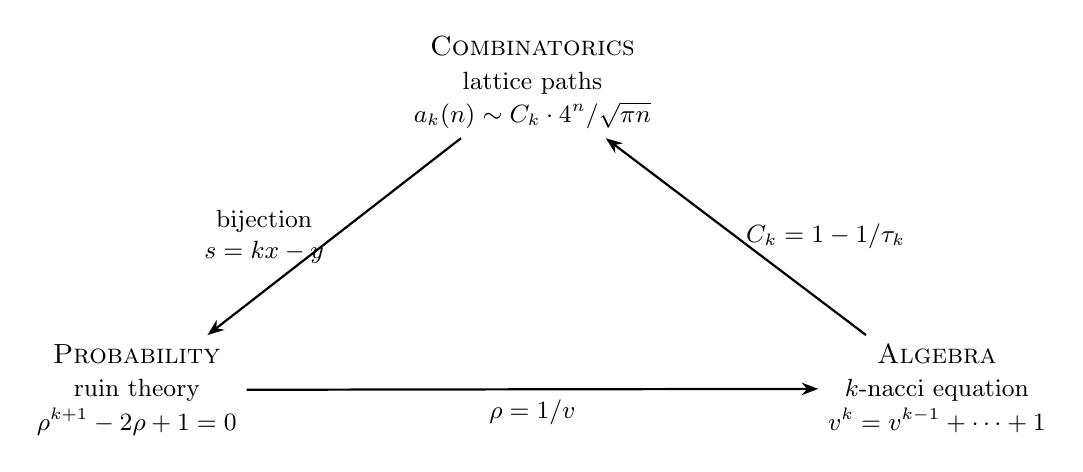
\begin{tikzpicture}[
  node distance=3.5cm,
  every node/.style={align=center},
  >={Stealth[length=6pt]}
]
\node (C) {\textsc{Combinatorics}\\{\small lattice paths}\\{\small $a_k(n) \sim C_k \cdot 4^n/\sqrt{\pi n}$}};
\node (P) [below left=2.5cm and 2cm of C]
  {\textsc{Probability}\\{\small ruin theory}\\{\small $\rho^{k+1} - 2\rho + 1 = 0$}};
\node (A) [below right=2.5cm and 2cm of C]
  {\textsc{Algebra}\\{\small $k$-nacci equation}\\{\small $v^k = v^{k-1} + \cdots + 1$}};

\draw[->, thick] (C) -- node[left, font=\small] {bijection\\$s = kx - y$} (P);
\draw[->, thick] (P) -- node[below, font=\small] {$\rho = 1/v$} (A);
\draw[->, thick] (A) -- node[right, font=\small] {$C_k = 1 - 1/\tau_k$} (C);
\end{tikzpicture}
\end{center}

\begin{example}[The golden ratio case, $k = 2$]\label{ex:golden}
The ruin equation is $\rho^3 - 2\rho + 1 = 0$, i.e.,
$(\rho - 1)(\rho^2 + \rho - 1) = 0$.
The sub-unit root is $\rho = (\sqrt{5} - 1)/2 = 1/\varphi$.
Hence $C_2 = 1 - 1/\varphi = 1/\varphi^2 = (3 - \sqrt{5})/2
\approx 0.382$.
\end{example}

\begin{example}[Degenerate case, $k = 1$]\label{ex:catalan}
The equation $\rho^2 - 2\rho + 1 = (\rho - 1)^2 = 0$ has a
double root at $\rho = 1$, giving $C_1 = 0$.
This is consistent with the Catalan asymptotics $a_1(n) \sim 4^n /
(\sqrt{\pi}\, n^{3/2})$: the coefficient of $4^n / \sqrt{\pi n}$
is zero, and the correct order is $4^n / n^{3/2}$ instead.
Probabilistically, $\rho = 1$ means certain ruin: the symmetric
$\{+1, -1\}$ walk returns to every level with probability~$1$.
\end{example}

\begin{corollary}[Limiting case]\label{cor:limit}
As $k \to \infty$, $\tau_k \to 2$ and
$C_k \to 1 - 1/2 = 1/2 = C_\infty$, consistent with the
unconstrained count $a_\infty(n) = \binom{2n-1}{n-1} \sim
4^n / (2\sqrt{\pi n})$.
\end{corollary}

\begin{remark}[Phase transition at $k = 1$]
The transition from $C_1 = 0$ to $C_2 = 1/\varphi^2 > 0$
is discontinuous in the following sense: for $k = 1$, the path count
has a \emph{qualitatively different} asymptotic form ($n^{-3/2}$
vs.\ $n^{-1/2}$).
In probabilistic language, this is the transition from
\emph{recurrent} ($k = 1$: the walk $\{+1, -1\}$ returns to every
state) to \emph{transient} ($k \geq 2$: the walk $\{+k, -1\}$ drifts
to $+\infty$).
\end{remark}

%======================================================================
\section{Rational slopes: the master equation}\label{sec:rational}
%======================================================================

For integer slopes, the random walk $\{+k, -1\}$ has uniform steps:
every position is equivalent.
For a rational slope $p/q$ with $p > q \geq 1$ and $\gcd(p, q) = 1$,
the Beatty staircase $S(x) = \floor{qx/p}$ has a periodic pattern
of height increments within each period of length~$p$.
The corresponding random walk inherits this periodicity, leading to a
\emph{position-dependent} ruin problem.

\subsection{Sturmian walks}

Define the rise sequence $r_j = S(j+1) - S(j)$ for $j = 0, 1, 2, \ldots$
This is a Sturmian word on the alphabet $\{\floor{q/p}, \ceil{q/p}\}$
with period~$p$ and exactly $q$ rises summing to~$q$ in each
period~\cite{Lothaire2002}.

The bijection $s = S(x) \cdot p/q - y$ (generalizing $s = kx - y$ from
the integer case) transforms the lattice path constraint into a
random walk on $\Z$ with position-dependent steps: from phase
$j \in \{0, 1, \ldots, q-1\}$, a right-step contributes $+r_j$ and
an up-step contributes $-1$, where $r_j = \floor{p(j+1)/q} - \floor{pj/q}$.

\subsection{Periodic ruin recursion}

The ruin probability now depends on the phase.
Let $\rho(s, j)$ be the ruin probability from position~$s$ in
phase~$j$.
The exponential ansatz $\rho(s, j) = A_j \cdot t^s$ gives the
amplitude relation
\[
\frac{A_{j+1}}{A_j} = \frac{2t - 1}{t^{r_j + 1}},
\]
where the factor arises from conditioning on the first step in the
symmetric case $p = q = 1/2$.

Requiring periodicity $A_{q} = A_0$ (the walk returns to the same
phase after $q$ steps) gives the \textbf{master equation}:

\begin{theorem}[Master equation]\label{thm:master}
The exponential rate $t$ of the ruin probability for the Sturmian walk
with slope $p/q$ satisfies
\begin{equation}\label{eq:master}
(2t - 1)^q = t^{p+q}.
\end{equation}
\end{theorem}

\begin{proof}
The product of amplitude ratios around one full period is
\[
\prod_{j=0}^{q-1} \frac{A_{j+1}}{A_j}
= \prod_{j=0}^{q-1} \frac{2t - 1}{t^{r_j + 1}}
= \frac{(2t-1)^q}{t^{\sum_j (r_j + 1)}}
= \frac{(2t-1)^q}{t^{p + q}},
\]
using $\sum_{j=0}^{q-1} r_j = p$ (total rise in one period) and
$\sum_{j=0}^{q-1} 1 = q$.
Setting this equal to~$1$ gives~\eqref{eq:master}.
\end{proof}

\begin{corollary}[Reduction to $k$-nacci]\label{cor:integer-collapse}
For integer slope $k$ (i.e., $q = 1$): $(2t-1)^1 = t^{k+1}$,
that is, $t^{k+1} - 2t + 1 = 0$, which is
equation~\eqref{eq:ruin-symmetric}.
\end{corollary}

\subsection{Roots and boundary system}

After removing the trivial root $t = 1$, equation~\eqref{eq:master}
has degree $p + q - 1$.

\begin{proposition}\label{prop:q-roots}
The master equation has exactly $q$ roots with $|t| < 1$.
\end{proposition}

This has been verified computationally for all coprime pairs $(p, q)$
with $p + q \leq 12$.
A proof via Rouch\'e's theorem applied to the sectors of the unit
disk is in preparation.

Let $t_1, \ldots, t_q$ denote the sub-unit roots.
The general solution of the ruin recursion is
\[
\rho(s, j) = \sum_{i=1}^{q} c_i \cdot A_j^{(i)} \cdot t_i^s,
\]
where the phase amplitudes $A_j^{(i)}$ (with $A_0^{(i)} = 1$) are
\begin{equation}\label{eq:amplitudes}
A_j^{(i)} = \prod_{m=0}^{j-1} \frac{2t_i - 1}{t_i^{r_m + 1}}.
\end{equation}
The boundary conditions $\rho(-1, j) = 1$ for $j = 0, \ldots, q - 1$
give a $q \times q$ linear system
\begin{equation}\label{eq:boundary}
\sum_{i=1}^{q} c_i \cdot \frac{A_j^{(i)}}{t_i} = 1,
\qquad j = 0, \ldots, q - 1.
\end{equation}

\begin{definition}
The asymptotic constant for rational slope $p/q$ is
\begin{equation}\label{eq:C-rational}
C(p/q) = \frac{1 - \sum_{i=1}^{q} c_i \cdot A_{j_0}^{(i)} \cdot
t_i^{s_0}}{2},
\end{equation}
where $s_0 = \floor{p/q}$ and $j_0 = 1 \bmod q$ (since the path
starts at $x = 1$, giving phase $1$, not~$0$).
\end{definition}

Since the $t_i$ are algebraic (roots of a polynomial with integer
coefficients), the amplitudes~\eqref{eq:amplitudes} and boundary
coefficients~\eqref{eq:boundary} are algebraic, and therefore:

\begin{theorem}\label{thm:algebraic}
For every rational slope $p/q$ with $p > q \geq 1$ and
$\gcd(p, q) = 1$, the asymptotic constant $C(p/q)$ is an algebraic
number.
\end{theorem}

\subsection{Example: slope 3/2}

For slope $3/2$ (the simplest non-integer case), the rise sequence is
$(r_0, r_1) = (1, 2)$: the staircase alternates between a step of
height~$1$ and a step of height~$2$.

The master equation $(2t - 1)^2 = t^5$ has degree~$5$; after
removing $t = 1$, it factors as $t^4 + 2t^3 - 2t^2 - 2t + 1 = 0$.
This palindromic quartic has two sub-unit roots (one pair of complex
conjugates).

The boundary system is $2 \times 2$.
Solving it and computing $C(3/2)$ yields an algebraic number of
degree~$6$ with minimal polynomial
\begin{equation}\label{eq:C32-poly}
x^6 - 10x^5 + 39x^4 - 69x^3 + 39x^2 - 10x + 1 = 0.
\end{equation}
The coefficients $(1, -10, 39, -69, 39, -10, 1)$ are
\emph{palindromic}: reading the polynomial backwards gives the same
polynomial.

\begin{remark}[Palindromic symmetry]
The palindromic structure of~\eqref{eq:C32-poly} means that if $C$
is a root, then so is $1 - C$.
This has a natural probabilistic interpretation: the symmetry
$C \leftrightarrow 1 - C$ corresponds to exchanging ``paths that
stay below'' and ``paths that cross'' the barrier.
Whether the minimal polynomial of $C(p/q)$ is palindromic for all
rational slopes is an open question.
\end{remark}

\subsection{Verification}

\begin{center}
\begin{tabular}{ccccc}
\toprule
Slope $p/q$ & $q$ & $C$ (ruin theory) & $C$ (numerical, 300 terms)
  & agreement \\
\midrule
$3/2$ & 2 & $0.251848165836$ & $0.251848165836$ & $20+$ digits \\
$5/2$ & 2 & $0.412376117412$ & $0.412376117412$ & $29$ digits \\
$5/3$ & 3 & $0.284123009123$ & $0.284123009123$ & $22$ digits \\
$7/3$ & 3 & $0.398094901320$ & $0.398094901320$ & $27$ digits \\
$4/3$ & 3 & $0.190858929$ & $0.190858929$ & $10$ digits \\
$7/4$ & 4 & $0.295424544708$ & $0.295424544708$ & $20$ digits \\
\bottomrule
\end{tabular}
\end{center}

Slopes near $k = 1$ (such as $4/3$, $5/4$) have slower Richardson
convergence in the numerical estimate, reducing the number of
matching digits.
The ruin-theoretic values are exact (algebraic).

\subsection{Collapse test}

When the rational slope $p/q$ happens to equal an integer $k$ (i.e.,
$p = kq$ with $q > 1$, not in lowest terms), the master equation
$(2t-1)^q = t^{(k+1)q}$ factors as
\[
2t - 1 = \omega^j \cdot t^{k+1},
\qquad j = 0, \ldots, q - 1,
\]
where $\omega = e^{2\pi i / q}$.
Only $j = 0$ gives the original equation $t^{k+1} - 2t + 1 = 0$;
the ``rotated'' roots for $j \neq 0$ produce oscillating phase
amplitudes and are eliminated by the boundary system.
The result correctly reduces to $C(k)$.

\emph{Verified:} slope $4/2 \to C(2) = 1/\varphi^2$,
slope $6/3 \to C(2) = 1/\varphi^2$, slope $6/2 \to C(3)$.

%======================================================================
\section{The fractal function \texorpdfstring{$C(\alpha)$}{C(α)}}
  \label{sec:fractal}
%======================================================================

The asymptotic constant $C(\alpha)$ can be viewed as a function of the
slope $\alpha \in (1, \infty)$.
Its basic properties are:

\begin{enumerate}
\item \textbf{Monotonicity:} $C$ is strictly increasing.
\item \textbf{Boundary values:} $C(1) = 0$ and
  $\lim_{\alpha \to \infty} C(\alpha) = 1/2$.
\item \textbf{Algebraic at rationals:} $C(p/q) \in \overline{\Q}$ for
  every rational $p/q > 1$ (Theorem~\ref{thm:algebraic}).
\item \textbf{Kink hierarchy:} $C$ has a kink (corner) at every
  rational point, with the kink magnitude governed by the denominator.
  At irrationals, $C$ is smooth.
\end{enumerate}

\subsection{Approximation by convergents}

For irrational $\alpha$ with convergents $p_k/q_k$, the algebraic
values $C(p_k/q_k)$ approximate $C(\alpha)$ from alternating sides.
The convergence is super-geometric.

\begin{example}[$\alpha = \varphi$, golden ratio]
The Fibonacci convergents $2/1, 3/2, 5/3, 8/5, 13/8, \ldots$ give:

\smallskip
\begin{center}
\begin{tabular}{ccccc}
\toprule
$k$ & $p_k/q_k$ & side & $|C(p_k/q_k) - C(\varphi)|$ & ratio \\
\midrule
2 & $2/1$ & above & $1.1 \times 10^{-1}$ & --- \\
3 & $3/2$ & below & $1.6 \times 10^{-2}$ & --- \\
4 & $5/3$ & above & $1.6 \times 10^{-2}$ & $0.14$ \\
5 & $8/5$ & below & $9.2 \times 10^{-4}$ & $0.057$ \\
6 & $13/8$ & above & $1.8 \times 10^{-3}$ & $0.11$ \\
7 & $21/13$ & below & $1.7 \times 10^{-5}$ & $0.018$ \\
\bottomrule
\end{tabular}
\end{center}

\smallskip\noindent
Same-side ratios are not constant but \emph{decrease}, indicating
super-geometric convergence.
The asymmetry (overshoot from above $\approx 2\times$ undershoot from
below) reflects the Sturmian correction structure.
\end{example}

\subsection{The hierarchy of defining equations}

Each slope type has a progressively more complex defining object for $C$:

\begin{center}
\begin{tabular}{llll}
\toprule
Slope & Defining equation for $C$ & Type & Complexity \\
\midrule
Integer $k$ & $\rho^{k+1} - 2\rho + 1 = 0$ & polynomial & degree $k$ \\
Rational $p/q$ & $(2t-1)^q = t^{p+q}$ + boundary & polynomial system &
  degree $p+q-1$ \\
Irrational & ??? & ??? & ??? \\
\bottomrule
\end{tabular}
\end{center}

For irrational slopes, the periodicity argument that produces the
master equation breaks down: the Sturmian word is aperiodic, the
transfer operator becomes infinite-dimensional, and the
``$q \times q$ boundary system'' has $q = \infty$.
Whether $C(\alpha)$ remains algebraic, or whether the
integer-to-rational transition (low-degree algebraic $\to$
higher-degree algebraic) is followed by an algebraic-to-transcendental
transition at irrational slopes, is the central open question.

%======================================================================
\section{Concluding remarks}\label{sec:outlook}
%======================================================================

\subsection{Summary of connections}

The identity $C_k = 1 - 1/\tau_k$ and its rational-slope extension
via the master equation $(2t-1)^q = t^{p+q}$ create a network of
connections between areas that have been studied largely independently:

\begin{itemize}
\item \textbf{Lattice paths $\leftrightarrow$ Ruin theory:}
  The bijection $s = kx - y$ (Section~\ref{subsec:ruin-lattice})
  transforms the combinatorial counting problem into a
  probabilistic survival problem.
  This connection was implicit in the work of Banderier and
  Flajolet~\cite{BanderierFlajolet2002} but, to our knowledge, the
  explicit identification of the ruin equation with the $k$-nacci
  equation has not appeared in the literature.

\item \textbf{Ruin theory $\leftrightarrow$ Multinacci constants:}
  The substitution $v = 1/\rho$ transforms the ruin equation
  $\sum \rho^j = 2$ into the $k$-nacci equation
  $v^k = v^{k-1} + \cdots + 1$.
  The ruin probability is $\rho = 1/\tau_k$.

\item \textbf{Multinacci constants $\leftrightarrow$ Lattice paths:}
  Each $k$-nacci constant determines the asymptotic
  constant of a lattice path sequence, and conversely, lattice path
  enumeration provides a combinatorial construction of Pisot numbers.

\item \textbf{Sturmian words $\leftrightarrow$ Ruin theory:}
  For rational slopes, the Sturmian pattern of the staircase
  determines the position-dependent step structure of the ruin
  problem, leading to the master equation.

\item \textbf{Exact counts $\leftrightarrow$ Asymptotics:}
  The Beatty Ballot Theorem~\cite{PopelkaBeattyBallot2026} shows that
  exact ballot numbers $B(p,q)$ appear at convergent positions.
  The present work determines the asymptotic growth rate between
  those positions.
  Both results derive from the Sturmian structure of the staircase.
\end{itemize}

\subsection{Open questions}

\begin{enumerate}
\item \textbf{Irrational slopes.}
  What replaces the master equation for irrational~$\alpha$?
  For the golden ratio $\alpha = \varphi$, the Sturmian word is
  generated by the Fibonacci substitution $a \to ab$, $b \to a$.
  The transfer matrix product over Fibonacci-length segments satisfies
  a matrix recurrence, but its spectral properties as a defining
  object for $C(\varphi)$ remain unclear.

\item \textbf{Algebraicity.}
  Is $C(\varphi) \approx 0.26934$ algebraic or transcendental?
  More generally, does $C(\alpha)$ undergo an algebraic-to-transcendental
  transition at irrational slopes?

\item \textbf{Palindromic structure.}
  The minimal polynomial of $C(3/2)$ is palindromic (self-reciprocal).
  Does this hold for all rational slopes?
  If so, the palindromic symmetry $C \leftrightarrow 1 - C$ might
  encode a duality in the ruin problem.

\item \textbf{Degree growth.}
  For rational $p/q$, the degree of the minimal polynomial of $C(p/q)$
  is bounded by the degree of the master equation ($p + q - 1$) but can
  be larger (e.g., degree~6 for slope $3/2$ where $p + q - 1 = 4$).
  What determines the degree of the minimal polynomial?

\item \textbf{OEIS entries.}
  The lattice path sequences for $k \geq 3$ (Example~\ref{ex:first-terms})
  do not appear in the OEIS.
  Each entry would arrive with a rich algebraic context: the asymptotic
  constant is a known Pisot-related number, the generating function
  satisfies a known algebraic equation, and the sequence fits into
  a parametric family interpolating between the Catalan numbers
  and the unconstrained binomial coefficients.

\item \textbf{Spectral geometry.}
  The interior roots of the master equation (those with $|t| < 1$) form
  patterns in the complex plane that depend on the slope $p/q$.
  For $q = 1$ (integer slopes), all roots are real.
  For $q \geq 2$, complex roots appear, clustered near $\operatorname{Re}(t)
  = 1/2$.
  Understanding this spectral geometry --- particularly its behavior as
  $q \to \infty$ along convergents of an irrational slope --- may
  illuminate the irrational-slope question.
\end{enumerate}

%======================================================================
\section*{Acknowledgments}
%======================================================================

Computational experiments were performed in Wolfram Language using the
Orbit paclet~\cite{orbit-paclet}.

\bibliographystyle{plain}
\bibliography{references}

\end{document}
